%++++++++++++++++++++++++++++++++++++++++
% Don't modify this section unless you know what you're doing!
%\documentclass[letterpaper,12pt]{article}
\documentclass[a4paper]{article}
\usepackage{tabularx} % extra features for tabular environment
\usepackage{amsmath}  % improve math presentation
\usepackage{graphicx} % takes care of graphic including machinery
%\usepackage[margin=1in,letterpaper]{geometry} % decreases margins
\usepackage{cite} % takes care of citations
%\usepackage[final]{hyperref} % adds hyper links inside the generated pdf file
%\hypersetup{
%	colorlinks=true,       % false: boxed links; true: colored links
%	linkcolor=blue,        % color of internal links
%	citecolor=blue,        % color of links to bibliography
%	filecolor=magenta,     % color of file links
%	urlcolor=blue
%}
%++++++++++++++++++++++++++++++++++++++++
\usepackage{indentfirst}
\usepackage{tensor}
\usepackage{amssymb}
\allowdisplaybreaks
\usepackage{bm}
\newcommand{\at}[2][]{#1|_{#2}}
\newcommand\numberthis{\addtocounter{equation}{1}\tag{\theequation}}
\newcommand\norm[1]{\left\lVert#1\right\rVert}

% Python code, taken from:
% https://www.quora.com/What-is-the-optimal-way-to-include-Python-code-in-a-LaTeX-document
\usepackage{color}
\usepackage{listings}
\usepackage{setspace}
\definecolor{Code}{rgb}{0,0,0}
\definecolor{Decorators}{rgb}{0.5,0.5,0.5}
\definecolor{Numbers}{rgb}{0.5,0,0}
\definecolor{MatchingBrackets}{rgb}{0.25,0.5,0.5}
\definecolor{Keywords}{rgb}{0,0,1}
\definecolor{self}{rgb}{0,0,0}
\definecolor{Strings}{rgb}{0,0.63,0}
\definecolor{Comments}{rgb}{0,0.63,1}
\definecolor{Backquotes}{rgb}{0,0,0}
\definecolor{Classname}{rgb}{0,0,0}
\definecolor{FunctionName}{rgb}{0,0,0}
\definecolor{Operators}{rgb}{0,0,0}
\definecolor{Background}{rgb}{0.98,0.98,0.98}
\lstset{
    breaklines=true,
    postbreak=\mbox{\textcolor{red}{$\hookrightarrow$}\space}
}
\lstdefinelanguage{Python}{
numbers=left,
numberstyle=\footnotesize,
numbersep=1em,
xleftmargin=1em,
framextopmargin=2em,
framexbottommargin=2em,
showspaces=false,
showtabs=false,
showstringspaces=false,
frame=l,
tabsize=4,
% Basic
basicstyle=\ttfamily\small\setstretch{1},
backgroundcolor=\color{Background},
% Comments
commentstyle=\color{Comments}\slshape,
% Strings
stringstyle=\color{Strings},
morecomment=[s][\color{Strings}]{"""}{"""},
morecomment=[s][\color{Strings}]{'''}{'''},
% keywords
morekeywords={import,from,class,def,for,while,if,is,in,elif,else,not,and,or,print,break,continue,return,True,False,None,access,as,,del,except,exec,finally,global,import,lambda,pass,print,raise,try,assert},
keywordstyle={\color{Keywords}\bfseries},
% additional keywords
morekeywords={[2]@invariant,pylab,numpy,np,scipy},
keywordstyle={[2]\color{Decorators}\slshape},
emph={self},
emphstyle={\color{self}\slshape},
%
}
\linespread{1.3}
% Python code [end].

\usepackage{caption}
\captionsetup[lstlisting]{font={small}}
\renewcommand{\lstlistingname}{Algorithm}

% Fontsize of figure smaller than normalsize:
\captionsetup[figure]{font=small}
\captionsetup[table]{font=small}

\begin{document}

\title{Atari Breakout with\\$\text{LTL}_f/\text{LDL}_f$ Goals}
%\author{Ivan Bergonzani, Michele Cipriano, Armando Nania}
%\date{\today}
%\maketitle


\makeatletter
\let\thetitle\@title
\let\theauthor\@author
\let\thedate\@date
\makeatother

\begin{titlepage}
	\centering
    \vspace*{0.5 cm}
    
\includegraphics[scale = 0.75]{images/SapienzaLogo}\\[1.0 cm]	% University Logo

    \vspace*{-0.3cm}
    \textsc{\large Department of Computer, Control and\\Management Engineering}\\[2.0 cm]	% Department Name
    \vspace*{1.2cm}

    { \fontsize{20.74pt}{18.5pt}\selectfont\bfseries \thetitle \par } % title

    \vspace*{0.1cm}
    \textsc{\Large Elective in Artificial Intelligence:\\Reasoning Robots}\\[0.5 cm] % course name

    \vspace*{2.8cm}
	\begin{minipage}{0.4\textwidth}
		\begin{flushleft} \large
			\emph{Professor:}\\
			Giuseppe De Giacomo\\
            %Computer Science Department\\
		\end{flushleft}
	\end{minipage}~
	\begin{minipage}{0.4\textwidth}
		\begin{flushright} \large
			\emph{Students:} \\
            Ivan Bergonzani \\
			Michele Cipriano\\
            Armando Nania
            %Semester\\
		\end{flushright}

	\end{minipage}\\[2 cm]

    \vspace{0.2cm}
    \rule{\linewidth}{0.2 mm} \\[0.3 cm]
    \vspace*{-0.3cm}
    Academic Year 2017/2018
\end{titlepage}

\tableofcontents
\newpage


%\begin{abstract}
%In this experiment we studied a very important physical effect by measuring the
%dependence of a quantity $V$ of the quantity $X$ for two different sample
%temperatures.  Our experimental measurements confirmed the quadratic dependence
%$V = kX^2$ predicted by Someone's first law. The value of the %mystery parameter
%$k = 15.4\pm 0.5$~s was extracted from the fit. This value is
%not consistent with the theoretically predicted $k_{theory}=17.34$~s. We attribute this
%discrepancy to low efficiency of our $V$-detector.
%\end{abstract}


\section{Introduction}
Introduction to the whole project, structure of the report and summary of
the work.

\clearpage
\section{Reinforcement Learning}
Reinforcement learning \cite{Suttonrl18} is an area of machine learning
which aims at studying how to to develop agents that can interact with
their environment maximing a cumulative reward. The environment can be
formally defined as a Markov Decision Process (MDP), which is a tuple
$\langle S, A, \delta, R \rangle$ where $S$ is a finite state of states that can represent
the environment, $A$ is a finite state of actions that can be perform by
the agent in the environment, $\delta$ is a probability function modeling
the transition from a state to another when performing a certain action and
$R$ is a reward function which models the reward received by the environment
when performing a certain action which makes the agent move from a state
to another.

An interesting property of the MDP is that it satisfies the Markov property,
hence, the future states that will be reached by the agent do not depend
on the past interaction of the environment, but just on the current state.
This makes it possbile to define the transition and the reward function
depending only on the current state (and of course the action and the future
state of interest).

This section considers two common reinforcement learning algorithm,
namely Q-Learning and SARSA, which have been used in our experiments
in order to train an agent interacting with an Atari Breakout environment
(section \ref{subsec:experiments}).

\subsection{Q-Learning}
Q-Learning algorithm.
\begin{equation}
    Q(S_t, A_t) \leftarrow Q(S_t, A_t) + \alpha \Big[ R_{t+1} +
        \gamma \max_{a} Q(S_{t+1}, A_t) - Q(S_t, A_t) \Big]
\end{equation}

\lstinputlisting[caption=Q-Learning algorithm Python implementation.,
    language=Python]{implementation/TDBrain-QLearning.py}

\subsection{SARSA}
SARSA algorithm.
\begin{equation}
    Q(S_t, A_t) \leftarrow Q(S_t, A_t) + \alpha \Big[ R_{t+1} +
        \gamma Q(S_{t+1}, A_{t+1}) - Q(S_t, A_t) \Big]
\end{equation}

\lstinputlisting[caption=SARSA algorithm Python implementation.,
    language=Python]{implementation/TDBrain-Sarsa.py}

\clearpage
\section{$\text{LTL}_f/\text{LDL}_f$ Non-Markovian Rewards}
Intro.

\subsection{Theoretical Background}
Introduction to the research paper.

\subsection{Examples}
How it can be used to train a RL model.

\clearpage
\section{OpenAI Gym}
OpenAI \texttt{gym} \cite{1606.01540} is a toolkit for developing and comparing
reinforcement learning algorithms, without making assumptions about the
structure of the agent interacting with the environment, in order to
keep development flexible to updates on both sides.

\subsection{Framework}
The framework of \texttt{gym} allows to interact easily
with an environment, giving the developers to tools they need to perform
actions and to observe the state of the environment itself. In this way it is
possible to focus more on the development of the agent without spending
time on the structure of the world.

\texttt{gym} makes it possible to interact with multiple kinds of environments.
Among these, the authors of the framework developed the support for
Arcade Learning Environment \cite{bellemare13arcade}, which includes all the
classing Atari games, including Breakout, which has been used in this project.

\subsection{Examples}
Let's consider a simple example to understand how \texttt{gym} works and
how the framework can be used to interact with an environment.
The description will follow Algorithm \ref{lst:gym-breakout-example-py}.

\lstinputlisting[caption={Example of a random interaction with the \texttt{gym}
    environment \texttt{BreakoutNoFrameskip-v4}, used also in our experiments
    of subsection \ref{subsec:experiments}.},
    label={lst:gym-breakout-example-py},
    language=Python]{implementation/gym-breakout-example.py}

Initially (line 1) the framework is imported. Then (line 3-4) an environment
is created specifying its name and initializing it. The program makes a
random agent interact randomly with the environment for 1000 episodes (lines
6-11) before closing the environment. Line 7 renders the current
observation of the environment on screen, line 8-9 performs a random action
between those available in this Brekout version, note that the method
\texttt{step} return an \texttt{observation} (shown in Fig.
\ref{fig:gym-breakout-image-example}), which is an array of pixels
that represent the current state of the environment, a \texttt{reward},
which is a value return by the game after performing the specified action
\texttt{action}, a boolean value \texttt{done}, which is \texttt{True} is
the game is over, \texttt{False} otherwise, and \texttt{info} which contains
extra information about the game. Lines 10-11 handles the case when the game
is over, resetting the environment.

\begin{figure}
    \centering
    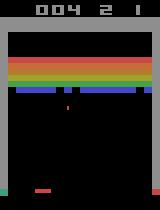
\includegraphics[width=0.3\textwidth]{images/gym-breakout-image-example.jpg}
    \caption{Observation of a frame of the environment
        \texttt{BreakoutNoFrameskip-v4}.}
    \label{fig:gym-breakout-image-example}
\end{figure}

\clearpage
\section{Atari Breakout}
Intro.

\subsection{PyGame Breakout}
Original implementation of the paper (non-ATARI).

\subsection{Arcade Learning Environment}
ATARI Breakout (from ALE) and differences from the other one.

\subsection{Implementation}
Intro to implementation.

\subsubsection{Robot Features Extractor}
\texttt{RobotFeatureExtractor} (OpenCV). Extracts features of the robot (robot
and ball positions).
\lstinputlisting[caption=Robot feature extractor Python implementation.,
    language=Python]{implementation/breakoutfull-breakoutrobotfeatureextractor.py}

\subsubsection{Goal Features Extractor}
\texttt{GoalFeatureExtractor} (OpenCV). Extracts 6x18 table representation
of the bricks in order to evaluate a formula.
\lstinputlisting[caption=Goal feature extractor Python implementation.,
    language=Python]{implementation/breakoutfull-breakoutgoalfeatureextractor.py}

\texttt{*Ext} used to improve implementation.

\subsubsection{Temporal Goals}
$\text{LTL}_f/\text{LDL}_f$ implementation (with Marco Favorito libraries).
\lstinputlisting[caption=$\text{LTL}_f/\text{LDL}_f$ formulas Python implementation.,
    language=Python]{implementation/breakoutfull-breakoutcompleterowstemporalevaluator.py}

Atari wrappers (OpenAI).

\subsection{Experiments}
\label{subsec:experiments}
Results with 6x18 non-ATARI Breakout (+CODE).

Results with our experiments (+CODE).

\clearpage
\section{Conclusion}
Why it does not work.

Summary + differences between the two environments.

Future works (neural networks and parallel computation).

%++++++++++++++++++++++++++++++++++++++++
% References section will be created automatically
% with inclusion of "thebibliography" environment
% as it shown below. See text starting with line
% \begin{thebibliography}{99}
% Note: with this approach it is YOUR responsibility to put them in order
% of appearance.

\clearpage
\bibliography{bibliography}
\bibliographystyle{ieeetr}

%\begin{thebibliography}{99}

%\bibitem{melissinos}
%A.~C. Melissinos and J. Napolitano, \textit{Experiments in Modern Physics},
%(Academic Press, New York, 2003).

%\bibitem{Cyr}
%N.\ Cyr, M.\ T$\hat{e}$tu, and M.\ Breton,
% "All-optical microwave frequency standard: a proposal,"
%IEEE Trans.\ Instrum.\ Meas.\ \textbf{42}, 640 (1993).

%\bibitem{Wiki} \emph{Expected value},  available at
%\texttt{http://en.wikipedia.org/wiki/Expected\_value}.

%\end{thebibliography}


\end{document}
